% Compile with: pdflatex -interaction=nonstopmode -halt-on-error
%                  -output-directory=output/pdf graph-informed-screening-proposal.tex
\documentclass[10pt,a4paper]{article}

\usepackage[T1]{fontenc}
\usepackage{lmodern}
\usepackage[a4paper,top=12mm,bottom=12mm,left=14mm,right=14mm]{geometry}
\usepackage{microtype}
\usepackage{amsmath,amssymb}
\usepackage{enumitem}
\usepackage{tikz}
\usepackage{xcolor}
\usepackage{titlesec}
\usepackage[hidelinks]{hyperref}

\definecolor{navy}{HTML}{18334C}
\definecolor{teal}{HTML}{A8D5CE}
\definecolor{purple}{HTML}{C9BEDA}
\definecolor{softgray}{HTML}{F2F4F5}
\definecolor{muted}{HTML}{52606A}

\pagestyle{empty}
\setlength{\parindent}{0pt}
\setlength{\parskip}{2.2pt}
\setlist[itemize]{leftmargin=4.3mm,itemsep=0.7pt,topsep=1.4pt,parsep=0pt}
\setlist[enumerate]{leftmargin=5.2mm,itemsep=0.7pt,topsep=1.4pt,parsep=0pt}
\titleformat{\section}{\color{navy}\bfseries\fontsize{10.8}{12}\selectfont}{}{0pt}{}
\titlespacing*{\section}{0pt}{4.2pt}{1.2pt}

\newcommand{\vsun}{\textsc{v.s.u.n.}}
\newcommand{\sectionrule}{\vspace{-1.5pt}{\color{navy!35}\hrule height .35pt}\vspace{1.2pt}}

\begin{document}
\fontsize{9.6}{11.1}\selectfont

\begin{center}
  {\color{navy}\bfseries\fontsize{16.2}{18}\selectfont
  Graph-Informed Screening for Stable and Novel Crystal Generation}\par
  \vspace{1.5pt}
  {\color{muted}\small Project Proposal}
\end{center}
\vspace{-3pt}

\section*{Project Motivation}
\sectionrule
The discovery of crystals with desirable physical properties enables advances in catalysis,
semiconductors, solar cells, batteries, and related technologies. De novo crystal generation seeks
to create entirely new structures using deep generative models, but evaluating the resulting search
space remains a bottleneck. Thermodynamic stability is most reliably assessed through formation-energy
comparisons and density functional theory (DFT), whose cost makes exhaustive evaluation of generated
crystals impractical. Generative models are therefore commonly judged using validity, stability,
uniqueness, and novelty (\vsun). High screening precision is essential: expensive validation should be
spent on candidates that are likely to be stable without collapsing generation toward already known
materials. Crys-JEPA shows that current models exhibit precisely this stability-novelty trade-off:
training toward dense, stable regions can reduce novelty, while moving away from known structures can
rapidly reduce stability~\cite{liu2026crysjepa}.

\section*{Project Description}
\sectionrule
Crys-JEPA addresses this bottleneck through an energy-aware embedding space in which crystals with
similar formation energies tend to lie close together. Its refinement pipeline (i) pre-trains a generator
on MP-20~\cite{xie2022cdvae}, (ii) generates candidates, relaxes them with a machine-learning force field
such as MatterSim~\cite{yang2024mattersim}, and retains candidates that are valid, unique, and novel,
(iii) retrieves training crystals from the candidate's chemical system and subsystems, and (iv) ranks
each candidate $C$ by the equal-weight mean embedding distance
\[
  D_C=\frac{1}{|R(C)|}\sum_{r\in R(C)}\lVert h_C-h_r\rVert_2^2.
\]
The lowest-distance fraction is fed back to fine-tune the generator~\cite{liu2026crysjepa}. This is an
effective DFT-free screening signal, but its reference pool has four limitations: it excludes potentially
transferable outside-system analogues; it weights references equally despite unequal relevance and
redundancy; it does not explicitly represent joint decomposition routes such as $AB+B$ for an $AB_2$
candidate; and its score depends on the size and composition of a fixed reference set.

\section*{Proposed Solution}
\sectionrule
We will study Crys-JEPA as a graph-structured representation and replace uniform reference aggregation
with candidate-conditioned, topology-aware screening. Same-system phases will remain the physically
valid competition set; outside-system crystals will provide learned structural or chemical context, not
be treated as literal decomposition products.

\noindent
\begin{minipage}[t]{0.66\textwidth}
\vspace{0pt}
\begin{enumerate}[label=\textbf{\arabic*.}]
  \item \textbf{Characterise the latent space.} Construct an embedding-space $k$-nearest-neighbour
  graph and use spectral and graph-theoretic analyses to identify clusters, low-density regions,
  connectivity, and local topology.
  \item \textbf{Probe encoded information.} Test whether neighbourhoods preserve properties beyond
  formation energy, including dielectric similarity where labels are available, and evaluate periodic,
  translation, and supercell invariance.
  \item \textbf{Learn reference relevance.} Expand the search pool using embedding, structural, and
  chemical similarity; then use graph-based weighting or a GNN aggregator to rank references and form
  a candidate-specific stability score. Redundant or weakly relevant references should receive less
  weight, while true competitors remain identifiable.
  \item \textbf{Evaluate controlled gains.} Compare the original restricted, equal-weight score with
  the expanded graph and learned weighting on the same generated pool and validation budget. Report
  screening precision and \vsun, and analyse cases that the graph method ranks highly despite a low
  baseline rank. Final claims of stability will use independent energy/hull validation rather than the
  learned score alone.
\end{enumerate}
\end{minipage}\hfill
\begin{minipage}[t]{0.31\textwidth}
\vspace{2pt}
\centering
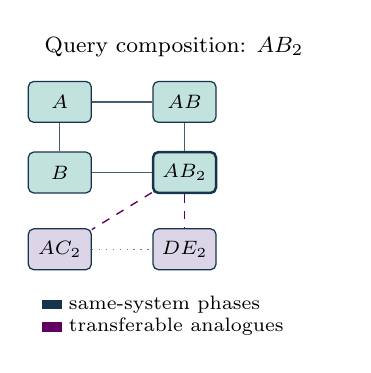
\begin{tikzpicture}[x=0.88cm,y=0.78cm,font=\scriptsize,
  node/.style={draw=navy,line width=.45pt,rounded corners=.7mm,minimum width=8mm,
               minimum height=5.2mm,inner sep=1pt},
  comp/.style={node,fill=teal!70},analog/.style={node,fill=purple!65}]
  \node[font=\footnotesize] at (2.0,4.15) {Query composition: $AB_2$};
  \node[comp] (a)  at (.35,3.25) {$A$};
  \node[comp] (ab) at (2.15,3.25) {$AB$};
  \node[comp] (b)  at (.35,2.10) {$B$};
  \node[comp,line width=.9pt] (ab2) at (2.15,2.10) {$AB_2$};
  \node[analog] (ac) at (.35,.85) {$AC_2$};
  \node[analog] (de) at (2.15,.85) {$DE_2$};
  \draw[navy!80,line width=.5pt] (a)--(ab)--(ab2)--(b)--(a);
  \draw[violet!75!black,dashed,line width=.5pt] (ab2)--(ac);
  \draw[violet!75!black,dashed,line width=.5pt] (ab2)--(de);
  \draw[navy!65,dotted,line width=.5pt] (ac)--(de);
  \node[align=left,anchor=north west,text width=3.7cm] at (-.05,.25)
    {\textcolor{navy}{\rule{2.5mm}{1.2mm}} same-system phases\\
     \textcolor{violet!75!black}{\rule{2.5mm}{1.2mm}} transferable analogues};
\end{tikzpicture}
\vspace{1pt}

{\color{muted}\scriptsize A broader reference graph preserves physical competitors while adding
context from nearby chemistries.}
\end{minipage}

\section*{Project Milestones}
\sectionrule
\begin{enumerate}[label=\textbf{M\arabic*.},leftmargin=7mm]
  \item A quantitative account of the structure, encoded properties, and invariances of the Crys-JEPA
  latent space.
  \item A graph-informed method for constructing reference pools and learning candidate-specific
  reference weights.
  \item A matched-budget evaluation demonstrating improved screening precision and \vsun\ for the
  generative-model refinement pipeline, together with interpretable ranking case studies.
\end{enumerate}

\clearpage
\fontsize{9.5}{11.5}\selectfont
\begin{thebibliography}{9}
\setlength{\itemsep}{5pt}

\bibitem{liu2026crysjepa}
N. Liu, N. Kazeev, S. G. Dale, et al.,
``Crys-JEPA: Accelerating Crystal Discovery via Embedding Screening and Generative Refinement,''
\emph{arXiv preprint arXiv:2605.14759}, 2026.
\url{https://arxiv.org/abs/2605.14759}

\bibitem{MatterGen2025}
C. Zeni, R. Pinsler, D. Z\"ugner, et al.,
``A generative model for inorganic materials design,''
\emph{Nature}, vol.~639, pp.~624-632, 2025.
\url{https://doi.org/10.1038/s41586-025-08628-5}

\bibitem{yang2024mattersim}
H. Yang, C. Hu, Y. Zhou, et al.,
``MatterSim: A Deep Learning Atomistic Model Across Elements, Temperatures and Pressures,''
\emph{arXiv preprint arXiv:2405.04967}, 2024.
\url{https://arxiv.org/abs/2405.04967}

\bibitem{xie2022cdvae}
T. Xie, X. Fu, O.-E. Ganea, R. Barzilay, and T. S. Jaakkola,
``Crystal Diffusion Variational Autoencoder for Periodic Material Generation,''
\emph{International Conference on Learning Representations (ICLR)}, 2022.
\url{https://arxiv.org/abs/2110.06197}

\end{thebibliography}

\end{document}
